\section{Experiments}
\subsection{Experimental Setup}
\textbf{Datasets}  
We use \textbf{PersonaMem} \citep{jiang2025know}, which includes multiple simulated user-LLM interaction histories over 7 real-world tasks, with memory lengths of 32K, 128K, and 1M tokens. 
Each history comprises up to 60 multi-turn sessions with evolving user personas and preferences. 
% PersonaMem supports multiple context lengths (32K, 128K, and 1M tokens) to challenge LLMs. 
We also evaluate on \textbf{PersonaBench} \citep{tan2025personabench}, a synthetic benchmark composed of private user documents and queries probing personal information (e.g., preferences, background), designed to assess the relevant personal memory retrieval ability before generation. 
And we include \textbf{LongMemEval} \citep{wu2024longmemeval}, a benchmark targeting long-term personalized retrieval, where factual questions require retrieving task-relevant information under both small and medium context settings. More details can be found at Appendix~\ref{app:dataset}. And \textbf{implementation details} can be found in Appendix~\ref{app:imple}

\textbf{Metrics}  
On PersonaMem, performance is measured by \emph{Accuracy} of generated responses, {i.e.}, the proportion of responses that correctly align with the user’s current persona and conversation context. On PersonaBench and LongMemEval, since the focus is on the retrieval of personal memory pieces, we use \emph{Recall@K} to assess how well relevant personal memories are retrieved.

\textbf{Baselines}  
Unlike prior baselines that often rely on LLM-generated queries or external indexing strategies, our comparisons are restricted to retrieval-only methods to ensure fairness: all systems operate on the same memory vectors. Since our focus is on the retrieval component itself, we compare RF-Mem against four direct baselines: 
\textbf{(1) Zero Memory}: Following~\citep{pan2025secom,jiang2025know}, the model answers without using user memory.
\textbf{(2) Full Context}: Following~\citep{pan2025secom,jiang2025know}, the entire user history memory is input to the model without retrieval. 
\textbf{(3) Dense Retrieval}: Following~\citep{wu2024longmemeval,pan2025secom,zhong2024memorybank}, a standard retriever that returns the top-$K$ memories based on similarity scores. This corresponds to the \emph{Familiarity} retrieval in dual-process theory. 
\textbf{(4) Recollection} (ours): The recollection mode we proposed in this paper. This represents the system that only enters the \emph{Recollection} path.



% \textbf{Metrics}  
% On PersonaMem, performance is measured by \emph{Accuracy} of generated responses, {i.e.}, the proportion of responses that correctly align with the user’s current persona and conversation context. On PersonaBench and LongMemEval, since the focus is on the retrieval of personal memory pieces, we use \emph{Recall@K} to assess how well relevant personal memories are retrieved.


% \begin{enumerate}
%   \item \textbf{Familiarity}: A standard vector retriever that directly returns the top-$k$ memory entries based on similarity scores, without any expansion or iterative refinement. This corresponds to the single-shot \emph{Familiarity} channel in dual-process theory.
%   \item \textbf{Recollection}: A purely slow retrieval mode where iterative clustering and query mixing are always applied, regardless of entropy. This represents a retrieval system that always enters the \emph{Recollection} channel, trading efficiency for thorough context reconstruction.
%   % \item \textbf{Ours — RF-Mem}: Our proposed dual-process framework that adaptively switches between Familiarity and Recollection according to entropy, aiming to balance efficiency and recall.
% \end{enumerate}

\subsection{Overall performance in Personalized Generation}

% 表格上就dense retrieval，(ours) 和(ours)， 加个discussion的适应性实验，画个简单的图，然后用rag的方法做实验。

% \begin{table}[ht]
% \vspace{-8pt}
% \centering
% \small
% \caption{Performance comparison \yy{over PersonaMem} across different memory corpus sizes. Columns are grouped by question type, rows by retrieval strategy. ``NA'' indicates the method does not need retrieval. ``OOC'' means out-of-context of the LLM input window. 
% % \yc{This table is not referred to and analyzed in the experiment part?}
% }
% \label{tab:personamem-alt}
% \setlength{\tabcolsep}{1pt}
%     \begin{tabular}{p{2.0cm}|M{1.0cm}|M{1.15cm}|M{1.2cm}M{1.4cm}M{0.9cm}M{1.2cm}M{1.3cm}M{1.0cm}M{1.0cm}|c}
%     \toprule
%      \textbf{Method} & \textbf{Retri Time}& \textbf{Avg. Tokens}&\textbf{Revisit Reasons} & \textbf{Track Evolution} & \textbf{Latest Prefs} & \textbf{Aligned Recs} & \textbf{New Scenarios}& \textbf{Shared Facts} & \textbf{New Ideas} & \textbf{Overall}  \\
%     \midrule
%     \rowcolor{gray!15}
%     \multicolumn{11}{c}{\textbf{32K memory corpus data}} \\
%     Zero Memory & NA &464.6 & 0.7273 &0.6259& 0.1765& 0.2182& 0.2105& 0.2326& 0.1183& 0.3854 \\
%     Full Context & NA &24657.8 & 0.9394&\textbf{0.7194}&\textbf{0.7647} &0.7455 &0.5614 &0.5039 &0.1828 &0.6129 \\
%     Dense Retrieval & 3.14ms&3515.9 & 0.9091 & 0.6475 & 0.6471 & 0.6364 & 0.5614 & 0.5426 & 0.2151 & 0.5908 \\
%     Recol. (ours) & 7.09ms &3711.1& \textbf{0.9495} & 0.6547 &0.7059 & \textbf{0.7818} & 0.5965 & 0.5194 & \textbf{0.2688} & 0.6214 \\
%     RF-Mem  (ours)& 5.09ms& 3566.6& \textbf{0.9495} & 0.6619 & 0.7059 & \textbf{0.7818} & \textbf{0.6140} & \textbf{0.5659} & \textbf{0.2688} & \textbf{0.6350} \\
%     \midrule
%     \rowcolor{gray!15}
%     \multicolumn{11}{c}{\textbf{128K memory corpus data}} \\
%     Zero Memory & NA &416.3 & 0.6766&0.6422&0.2136&0.2751&0.1925&0.2281&0.1737&0.3124 \\
%     Full Context & NA & 115601.4& 0.5613 &0.3930 &0.2783 &0.3868 &0.2770 &0.3977 &0.1795 &0.3231 \\
%     Dense Retrieval & 3.24ms & 3540.1 & 0.7881 & 0.6804 & 0.5346 & 0.5330 & 0.3662 & 0.6082 & 0.3069 & 0.5259 \\
%     Recol. (ours) & 7.86ms &3680.3& \textbf{0.8141} & 0.6716 & 0.5254 & 0.5301 & 0.3765 & 0.6140 & \textbf{0.3263} & 0.5288 \\
%     RF-Mem (ours)&4.27ms &3565.5& 0.8030 & \textbf{0.6862} & \textbf{0.5427} &\textbf{0.5358} & \textbf{0.4131} & \textbf{0.6257} &\textbf{ 0.3263} & \textbf{0.5394 }\\
%     \midrule
%     \rowcolor{gray!15}
%     \multicolumn{11}{c}{\textbf{1M memory corpus data}} \\
%     Zero Memory & NA & 415.1& 0.6000&0.6178&0.1797&0.3179&0.1831&0.2569&0.1816&0.2730 \\
%     Full Context & NA &912148.5 &OOC &OOC &OOC &OOC &OOC &OOC &OOC &OOC \\
%     Dense Retrieval& 4.42ms & 3816.1& 0.7702 & \textbf{0.6933} & \textbf{0.4544} & 0.4464 & 0.3085 & 0.5903 & 0.3040 & 0.4518 \\
%     Recol. (ours) & 7.12ms&3847.4 & 0.7532 & 0.6800 & 0.4440 & 0.4500 & \textbf{0.3593} & 0.5833 & 0.3136 & 0.4544 \\
%     RF-Mem (ours)& 6.28ms & 3827.8& \textbf{0.7787} & 0.6889 & 0.4492 & \textbf{0.4536} & 0.3390 & \textbf{0.6111} & \textbf{0.3150} & \textbf{0.4589} \\
%     \bottomrule
%     \end{tabular}
% % \vspace{-5pt}
% \end{table}

\vspace{-15pt}
\begin{table}[ht]
\centering
\small
\caption{Performance comparison \yy{over the PersonaMem} across different memory corpus sizes. Columns are grouped by question type, rows by retrieval strategy. ``NA'' indicates the method does not need retrieval. ``OOC'' means out-of-context of the LLM input window. The best results are in \textbf{bold}, and the second-best results are \underline{underlined}. ``\textbf{{\large *}}'' indicates the statistically significant improvements (i.e., two-sided t-test with $p<0.05$) over the best baseline. 
% \zxy{``\textbf{{\large *}}'' indicates the statistically significant improvements (i.e., two-sided t-test with $p<0.05$) over the best baseline. $\uparrow$: higher is better. $\downarrow$: lower is better.}
% \yc{This table is not referred to and analyzed in the experiment part?}
}
\label{tab:personamem-alt}
\setlength{\tabcolsep}{1pt}
\renewcommand{\arraystretch}{0.9}
    \begin{tabular}{p{2.0cm}|M{1.0cm}|M{1.15cm}|M{1.2cm}M{1.4cm}M{0.9cm}M{1.2cm}M{1.3cm}M{1.0cm}M{1.0cm}|>{\columncolor{blue!5}}c}
    \toprule
     \textbf{Method} & \textbf{Retri Time}& \textbf{Avg. Tokens}&\textbf{Revisit Reasons} & \textbf{Track Evolution} & \textbf{Latest Prefs} & \textbf{Aligned Recs} & \textbf{New Scenarios}& \textbf{Shared Facts} & \textbf{New Ideas} & \textbf{Overall}  \\
    \midrule
    \rowcolor{gray!15}
    \multicolumn{11}{c}{\textbf{32K memory corpus data}} \\
    Zero Memory & NA &464.6 & 0.7273 &0.6259& 0.1765& 0.2182& 0.2105& 0.2326& 0.1183& 0.3854 \\
    Full Context & NA &24657.8 & \underline{0.9394}&\textbf{0.7194}&\textbf{0.7647} &\underline{0.7455} &0.5614 &0.5039 &0.1828 &0.6129 \\
    Dense Retrieval & 3.14ms&3515.9 & 0.9091 & 0.6475 & 0.6471 & 0.6364 & 0.5614 & \underline{0.5426} & \underline{0.2151} & 0.5908 \\
    Recol. (ours) & 7.09ms &3711.1& \textbf{0.9495} & 0.6547 &0.7059 & \textbf{0.7818} & \underline{0.5965} & 0.5194 & \textbf{0.2688} & \underline{0.6214}\\
    RF-Mem  (ours)& 5.09ms& 3566.6& \textbf{0.9495} & \underline{0.6619} & \underline{0.7059} & \textbf{0.7818} & \textbf{0.6140} & \textbf{0.5659} & \textbf{0.2688} & \textbf{0.6350$^*$} \\
    \midrule
    \rowcolor{gray!15}
    \multicolumn{11}{c}{\textbf{128K memory corpus data}} \\
    Zero Memory & NA &416.3 & 0.6766&0.6422&0.2136&0.2751&0.1925&0.2281&0.1737&0.3124 \\
    Full Context & NA & 115601.4& 0.5613 &0.3930 &0.2783 &0.3868 &0.2770 &0.3977 &0.1795 &0.3231 \\
    Dense Retrieval & 3.24ms & 3540.1 & 0.7881 & \underline{0.6804} & \underline{0.5346} & \underline{0.5330} & 0.3662 & 0.6082 & 0.3069 & 0.5259 \\
    Recol. (ours) & 7.86ms &3680.3& \textbf{0.8141} & 0.6716 & 0.5254 & 0.5301 & \underline{0.3765} & \underline{0.6140} & \textbf{0.3263} & \underline{0.5288} \\
    RF-Mem (ours)&4.27ms &3565.5& \underline{0.8030} & \textbf{0.6862} & \textbf{0.5427} &\textbf{0.5358} & \textbf{0.4131} & \textbf{0.6257} &\textbf{ 0.3263} & \textbf{0.5394$^*$}\\
    \midrule
    \rowcolor{gray!15}
    \multicolumn{11}{c}{\textbf{1M memory corpus data}} \\
    Zero Memory & NA & 415.1& 0.6000&0.6178&0.1797&0.3179&0.1831&0.2569&0.1816&0.2730 \\
    Full Context & NA &912148.5 &OOC &OOC &OOC &OOC &OOC &OOC &OOC &OOC \\
    Dense Retrieval& 4.42ms & 3816.1& \underline{0.7702} & \textbf{0.6933} & \textbf{0.4544} & 0.4464 & 0.3085 & \underline{0.5903} & 0.3040 & 0.4518 \\
    Recol. (ours) & 8.12ms&3847.4 & {0.7532} & 0.6800 & 0.4440 & \underline{0.4500} & \textbf{0.3593} & 0.5833 & \underline{0.3136} & \underline{0.4544} \\
    RF-Mem (ours)& 6.28ms & 3827.8& \textbf{0.7787} & \underline{0.6889} & \underline{0.4492} & \textbf{0.4536} & \underline{0.3390} & \textbf{0.6111} & \textbf{0.3150} & \textbf{0.4589$^*$} \\
    \bottomrule
    \end{tabular}
% \vspace{-5pt}
\end{table}


% \begin{table}[h]
% \centering
% \small
% \caption{Performance comparison on different memory corpus sizes.}
% \label{tab:memory_corpus}
% \setlength{\tabcolsep}{1pt}
% \renewcommand{\arraystretch}{1.0}
% \begin{tabular}{p{2.5cm}M{1.1cm}M{1.1cm}M{1.2cm} | M{1.1cm}M{1.1cm}M{1.2cm}| M{1.1cm}M{1.1cm}M{1.2cm}}
% \toprule
% \multirow{2}{*}{\textbf{Question Category}} 
% & \multicolumn{3}{c}{\textbf{32k memory corpus}} 
% & \multicolumn{3}{c}{\textbf{128k memory corpus}} 
% & \multicolumn{3}{c}{\textbf{1M memory corpus}} \\
% \cmidrule(lr){2-4} \cmidrule(lr){5-7} \cmidrule(l){8-10}
% & Famili. & Recol. & RF-Mem 
% & Famili. & Recol. & RF-Mem 
% & Famili. & Recol. & RF-Mem  \\
% \midrule
% Overall          & 0.5908 & 0.6214 & \textbf{0.6350} & 0.5259 & 0.5288 & \textbf{0.5394 }& 0.4518 & 0.4544 & \textbf{0.4589} \\ 
% \midrule
% Home Decoration  & \textbf{0.6667} & \textbf{0.6667} & \textbf{0.6667} & 0.6275 & 0.6275 & \textbf{0.6471} & 0.4207 & \textbf{0.4451} & 0.4207 \\
% Family Relations & 0.5625 & \textbf{0.5938} & \textbf{0.5938} & 0.5486 & 0.5625 & \textbf{0.5764} & 0.5734 & 0.5803 & \textbf{0.6010} \\
% Therapy          & \textbf{0.5000} & \textbf{0.5000} & \textbf{0.5000} & 0.5060 & 0.5301 & \textbf{0.5341} & 0.4534 & \textbf{0.5280} & 0.4845 \\
% Travel Plan      & 0.4789 & \textbf{0.5775} & 0.5634 & 0.5806 & 0.6194 & \textbf{0.6452} & \textbf{0.4948} & 0.4792 & 0.4896 \\
% \midrule
% Medical Consult  & \textbf{0.8421} & 0.7895 & \textbf{0.8421} & 0.4718 & \textbf{0.5128} & 0.5026 & 0.4294 & 0.4110 & \textbf{0.4356} \\
% Legal Consult    & 0.7812 & 0.8750 & \textbf{0.9375} & \textbf{0.5124} & 0.4735 & 0.4841 & \textbf{0.4061} & 0.3909 & 0.3909 \\
% Study Consult    & \textbf{0.6000} & \textbf{0.6000} & \textbf{0.6000} & \textbf{0.5096} & 0.4904 & 0.4773 & 0.4503 & 0.4293 & \textbf{0.4817} \\
% Dating Consult   & 0.5851 & 0.5851 & \textbf{0.6277} & 0.4772 & \textbf{0.5025} & 0.4975 & \textbf{0.5192} & 0.5000 & 0.5096 \\
% Financial Consult& 0.5556 & 0.5972 & \textbf{0.6389} & 0.4899 & 0.4697 & \textbf{0.4899} & \textbf{0.4365} & 0.4309 & 0.4199 \\
% \midrule
% Food Rec         & \textbf{1.0000} & \textbf{1.0000} & \textbf{1.0000} & 0.5240 & \textbf{0.5721} & 0.5633 & 0.3717 & \textbf{0.4241} & 0.3874 \\
% Movie Rec        & \textbf{0.6154} & \textbf{0.6154} & 0.5865 & \textbf{0.5759} & 0.5696 & 0.5633 & 0.4434 & 0.4481 & \textbf{0.4575} \\
% Music Rec        & 0.6071 & \textbf{0.6250} & \textbf{0.6250} & 0.4091 & 0.4773 & \textbf{0.5096} & 0.4609 & 0.4688 & \textbf{0.5000 }\\
% Book Rec         & 0.5373 & 0.5970 & \textbf{0.6418} & 0.5640 & 0.5407 & \textbf{0.5814} & 0.4964 & 0.4532 & \textbf{0.5036} \\
% Sports Rec       &   -    &   -    &   -    & \textbf{0.5228} & 0.4670 & 0.4975 & 0.4189 & \textbf{0.4392} & \textbf{0.4392} \\
% Online Shopping  &   -    &   -    &   -    & 0.5408 & 0.5459 & \textbf{0.5561} & 0.3738 & \textbf{0.3932} & 0.3786 \\
% \bottomrule
% \end{tabular}
% \vspace{-5pt}
% \end{table}

% \begin{figure}[ht]
%     \centering
%     \includegraphics[width=0.98\linewidth]{iclr2026/chapter/figure/heatmaps.pdf}
%     \caption{Heatmap of Familiarity (Fami.), Recollection (Recool.), and RF-Mem across question categories under three memory corpus sizes.}
%     \label{fig:heatmaps}
% \end{figure}

% To verify the effectiveness of RF-Mem, we conduct experiments on \textbf{PersonaMem} across memory corpora of 32K, 128K, and 1M tokens for each query. This setup allows us to stress-test retrieval under different corpus scales and query types. The results in Table~\ref{tab:personamem-alt} clearly show that a single-process retriever is insufficient for personalized memory reasoning. Moreover, to further examine retrieval behaviors across tasks and corpus scales, we evaluate the three strategies on diverse question categories, ranging from fact-oriented queries (e.g., \emph{food recommendation}, \emph{medical consult}) to reasoning-intensive ones (e.g., \emph{study consult}, \emph{family relations}, \emph{new scenarios}). We also reports per-category accuracy under three corpus sizes in Table~\ref{tab:memory_corpus}.

To verify the effectiveness of RF-Mem, we evaluate it on \textbf{PersonaMem} across memory corpora of 32K, 128K, and 1M tokens per query. This setup stresses retrieval under different memory scales and question types, allowing us to examine how retrieval methods adapt as corpora grow larger and tasks become more complex. Table~\ref{tab:personamem-alt} compares zero-memory baselines, full-context input, and three retrieval strategies (Dense, Recollection, RF-Mem). 
% The results clearly demonstrate that single-mode retrievers struggle to maintain robustness under scaling, motivating the need for adaptive retrieval. 
We also report per-category accuracy under three corpus sizes in Appendix~\ref{app:cate_res} and different $K$ settings in Appendix~\ref{app:pm_k}.

\textbf{First, RF-Mem delivers the best \emph{overall} accuracy at every corpus scale while keeping inputs compact.} \yy{In Table~\ref{tab:personamem-alt}}, RF-Mem attains the top overall score at 32K (0.6350), 128K (0.5394), and 1M (0.4589). At 32K it surpasses Full Context by +0.0221 with only 3.6k average tokens versus 24.7k for Full Context, and with a modest 5.09ms retrieval time. As the memory grows, Full Context deteriorates sharply, reaching 0.3231 at 128K and becoming out of context at 1M, whereas RF-Mem remains stable and leads Dense Retrieval (Familarity) by +0.0135 at 128K and +0.0071 at 1M. These trends validate that when a question is familiar, RF-Mem saves budget; when unfamiliar, it upgrades to structured recollection without committing to the cost of running it unconditionally.

\textbf{Second, RF-Mem leads on hybrid and transfer-style tasks with lower overhead.} At 32K it achieves top scores on \emph{Aligned Recommendations} (0.7818), \emph{New Scenarios} (0.6140), and \emph{Shared Facts} (0.5659) , while remaining close on \emph{Track Evolution}. 
% At 128K it remains ahead on \emph{Track Evolution} (0.6862), \emph{Latest Prefs} (0.5427), \emph{Aligned Recs} (0.5358), \emph{New Scenarios} (0.4131), and \emph{Shared Facts} (0.6257), tying on \emph{New Ideas} (0.3263). 
At 128K it remains ahead on \emph{Track Evolution}, \emph{Latest Prefs}, \emph{Aligned Recs}, \emph{New Scenarios}, and \emph{Shared Facts}, tying on \emph{New Ideas}. 
At 1M, where Full Context is infeasible, RF-Mem is strongest on \emph{Revisit Reasons}, \emph{Aligned Recs}, \emph{Shared Facts}, and \emph{New Ideas}, with only small gaps on \emph{Track Evolution} and \emph{Latest Prefs}, indicating that adaptive depth better balances precise anchoring and selective expansion than single-mode retrieval.

\textbf{Third, RF-Mem achieves a favorable accuracy–efficiency trade-off by regulating retrieval depth via entropy.} Compared to always-on recollection, RF-Mem improves overall accuracy while reducing latency: 5.09ms vs 7.09ms at 32K, 4.27ms vs 7.86ms at 128K, and 6.28ms vs 7.12ms at 1M, with similar token budgets to Dense Retrieval. This efficiency arises from treating familiarity as the default and route to the recollection path only when the question is unfamiliar. The result is a scalable retrieval controller that avoids the out-of-context cliff of Full Context, outperforms dense retrieval baselines as memory scales, and preserves recollection’s advantages precisely.

% \textbf{First, Familiarity excels in direct recall but degrades under complexity.} 
% Across corpus sizes, in Table~\ref{tab:personamem-alt}, the Familiarity path maintains strong performance on fact-centric tasks such as ``Shared Facts'' and ``Revisit Reasons,'' consistent with its cognitive role of providing a fast, coarse recognition signal. However, as tasks demand longer reasoning chains (e.g., ``Track Evolution,'' ``Aligned Recommendations''), Familiarity’s one-shot retrieval shows clear limitations, particularly when the memory scale increases. 

% \textbf{Second, Recollection benefits complex reasoning but incurs instability.} 
% In Table~\ref{tab:personamem-alt}, Recollection consistently improves on reasoning-intensive tasks that require context reconstruction, validating its role as the “slow but diagnostic” channel in dual-process theory. Yet, this advantage comes at the cost of efficiency and stability: on simpler queries or large memory corpora, Recollection often underperforms due to redundant expansion. 

% \textbf{Third, grounded in dual-process theory, RF-Mem unifies the two retrieval channels through entropy-driven selection.} 
% By dynamically switching between Familiarity and Recollection, RF-Mem preserves the efficiency of fast recognition when confidence is high, while activating deliberate recollection only when uncertainty necessitates deeper exploration. 
% In Table~\ref{tab:personamem-alt}, this dual-process regulation yields consistent gains across both task types and corpus scales, highlighting entropy-aware switching as essential for scalable personalized memory retrieval. 

% This advantage is confirmed in Table~\ref{tab:memory_corpus}, where Familiarity achieves peak accuracy in rec categories such as \emph{food recommendation} (1.0000 at 32k corpus) and \emph{movie recommendation} (0.5759 at 128k corpus), showing that surface-level matches are often sufficient for direct factual retrieval. 
% In contrast, its effectiveness diminishes in consultative domains such as \emph{family relations}, \emph{therapy}, and \emph{legal consult}, where deeper reasoning is required. 

% Table~\ref{tab:memory_corpus} further illustrates this contrast across task categories. 
% In consultative domains such as \emph{family relations}, \emph{therapy}, and \emph{dating consultation}, Recollection surpasses Familiarity by integrating broader contextual evidence. Yet in factual categories like \emph{food recommendation} or \emph{study consultation}, where surface-level matches suffice, Recollection provides little or no gain. 

% Furthermore, in Table~\ref{tab:memory_corpus}, category-level analysis shows that RF-Mem particularly excels in hybrid tasks such as \emph{aligned recommendations} and \emph{new scenarios}, where low-confidence probes benefit from recollection. 
% Unlike single-mode strategies that degrade at the million-scale corpus, RF-Mem sustains stable accuracy by adapting its retrieval depth, confirming its advantage in capturing key user memories without committing to a fixed strategy.

% Its instability also appears in recommendation-oriented tasks such as \emph{book} and \emph{music recommendation}, where performance fluctuates across corpus scales. 
% This pattern directly reflects the dual-process theory: fast Familiarity captures salient cues efficiently, while slow Recollection is indispensable for deeper reasoning, albeit at the cost of robustness under scale.

% \begin{table}[t]
% \centering
% \small
% \caption{Performance comparison across different memory corpus sizes. Fam. = Familiarity, Rec. = Recollection.}
% \label{tab:personamem-results}
% \setlength{\tabcolsep}{4pt}
% \renewcommand{\arraystretch}{1.1} %可以控制行间距
% % \resizebox{140mm}{!}{
%     \begin{tabular}{l|ccc|ccc|ccc}
%     \toprule
%     \multirow{2}{*}{\textbf{Question Type}} & \multicolumn{3}{c|}{\textbf{32K memory data}} & \multicolumn{3}{c|}{\textbf{128K memory data}} & \multicolumn{3}{c}{\textbf{1M memory data}} \\
%     & Fam. & Rec. & RF-Mem & Fam. & Rec. & RF-Mem & Fam. & Rec. & RF-Mem \\
%     \midrule
%     Revisit Reasons & 0.9091 & 0.9495 & 0.9394 & 0.7881 & 0.8141 & 0.8030 & 0.7702 & 0.7617 & 0.7702 \\
%     Track Evolution& 0.6475 & 0.6763 & 0.6547 & 0.6804 & 0.6716 & 0.6862 & 0.6933 & 0.6844 & 0.7067 \\
%     Latest Prefs & 0.6471 & 0.7059 & 0.7059 & 0.5346 & 0.5254 & 0.5427 & 0.4544 & 0.4674 & 0.4622 \\
%     Aligned Recs& 0.6364 & 0.7273 & 0.7636 & 0.5330 & 0.5301 & 0.5358 & 0.4464 & 0.4321 & 0.4464 \\
%     New Scenarios& 0.5614 & 0.6140 & 0.6316 & 0.3662 & 0.3765 & 0.4131 & 0.3085 & 0.3288 & 0.3153 \\
%     Shared Facts & 0.5426 & 0.6047 & 0.6124 & 0.6082 & 0.6140 & 0.6257 & 0.5903 & 0.5764 & 0.5833 \\
%     New Ideas & 0.2151 & 0.1828 & 0.2151 & 0.3069 & 0.3263 & 0.3263 & 0.3040 & 0.3177 & 0.3136 \\ 
%     \midrule
%     Overall & 0.5908 & 0.6282 & 0.6333 & 0.5259 & 0.5288 & 0.5394 & 0.4518 & 0.4577 & 0.4581 \\
%     \bottomrule
%     \end{tabular}
% % }
% \end{table}

% To verify the effectiveness of RF-Mem, we conduct experiments on \textbf{PersonaMem} across memory corpora of 32K, 128K, and 1M. This setup allows us to stress-test retrieval under different scales memory corpus and query types. The results in Table~\ref{tab:personamem-alt} provide clear evidence that a single-process retriever is insufficient for personalized memory reasoning.

% \textbf{First, Familiarity excels in direct recall but degrades under complexity.} 
% Across corpus sizes, the Familiarity path maintains strong performance on fact-centric tasks such as ``Shared Facts'' and ``Revisit Reasons,'' consistent with its cognitive role of providing a fast, coarse recognition signal. 
% However, as tasks demand longer reasoning chains (e.g., ``Track Evolution,'' ``Aligned Recommendations''), Familiarity’s one-shot retrieval shows clear limitations, particularly when the memory scale increases.  

% \textbf{Second, Recollection benefits complex reasoning but incurs instability.} 
% Recollection consistently improves on reasoning-intensive tasks that require context reconstruction, validating its role as the “slow but diagnostic” channel in dual-process theory. 
% Yet, this advantage comes at the cost of efficiency and stability: on simpler queries or large memory corpora, Recollection often underperforms due to redundant expansion and higher variance.  

% \textbf{Third, RF-Mem unifies the two channels through dynamic selection.} 
% By adaptively switching based on entropy, RF-Mem preserves the efficiency of Familiarity where confidence is high, while invoking Recollection only when uncertainty demands deeper exploration. 
% This dual-process regulation yields stable gains across both task types and corpus scales, confirming that uncertainty-aware switching is crucial for scalable personalized memory retrieval.  



% To further examine retrieval behaviors across tasks and memory scales, we evaluate Familiarity, Recollection, and RF-Mem on diverse question categories, ranging from fact-oriented queries (e.g., \emph{food recommendation}, \emph{medical consult}) to reasoning-intensive ones (e.g., \emph{study consult}, \emph{family relations}, \emph{new scenarios}). Figure~\ref{fig:heatmaps} reports per-category accuracy under three corpus sizes (32K, 128K, 1M), visualized as heatmaps for intuitive comparison. 

% \textbf{Familiarity excels at direct recall tasks while Recollection dominates reasoning-heavy queries.} 
% As shown in Figure~\ref{fig:heatmaps}, Familiarity achieves strong results in straightforward factual categories such as \emph{food recommendation} and \emph{legal consultation}, where surface-level matches suffice. In contrast, Recollection consistently outperforms in tasks requiring broader context reconstruction, such as \emph{study consultation}, \emph{family relations}, and \emph{travel planning}. This contrast reflects the dual-process theory: fast familiarity captures salient cues, while slow recollection is necessary for integrating distributed contextual evidence.

% \textbf{RF-Mem achieves robust performance by dynamically balancing the two retrieval modes.} 
% Across corpus scales, RF-Mem adaptively switches strategies, outperforming both baselines in categories such as \emph{aligned recommendations} and \emph{new scenarios}, where low-confidence probes benefit from deliberate recollection. Moreover, while single-mode strategies degrade as the memory corpus grows to one million entries, RF-Mem sustains stable accuracy by leveraging entropy-driven regulation. This confirms that RF-Mem reliably captures key user memories through uncertainty-aware adaptation rather than committing to a fixed retrieval strategy.

\subsection{Overall performance in Personalized Retrieval}

\begin{table}[ht]
\vspace{-10pt}
\centering
\small
\caption{Performance comparison over the PersonaBench dataset across multiple question types. The best results are in \textbf{bold}, and the second-best results are \underline{underlined}.}
\label{tab:personabench}
\setlength{\tabcolsep}{1.3pt}
\renewcommand{\arraystretch}{1.0}
    \resizebox{140mm}{!}{
    \begin{tabular}{p{1.3cm}|M{1.05cm}M{0.9cm}M{0.9cm}M{0.9cm}M{0.9cm}>{\columncolor{blue!5}}M{1.0cm}|M{1.05cm}M{0.9cm}M{0.9cm}M{0.9cm}M{0.9cm}>{\columncolor{blue!5}}M{1.0cm}}
        \toprule
        \textbf{Metrics}  &
        \multicolumn{6}{c|}{\textbf{Recall@5}} &
        \multicolumn{6}{c}{\textbf{Recall@10}} \\
        \cmidrule(lr){2-7} \cmidrule(l){8-13}
        \textbf{Method} 
        & \textbf{Time} & \textbf{Basic Info} & \textbf{Social Info} & \textbf{Pref Easy} & \textbf{Pref Hard} & \textbf{Overall}   
        & \textbf{Time}& \textbf{Basic Info} & \textbf{Social Info} & \textbf{Pref Easy} & \textbf{Pref Hard} & \textbf{Overall}   \\
        \midrule
        \rowcolor{gray!15}
        \multicolumn{13}{c}{\textit{multi-qa-MiniLM-L6-cos-v1}} \\
        Famili. & 8.40ms & \underline{0.4515} & 0.4852 & \underline{0.4904}& \underline{0.3659} & 0.4484  & 13.68ms & \underline{0.5879} & 0.6220 & \textbf{0.6442} & \underline{0.5561} & 0.5964  \\
        Recol.  & 9.65ms & 0.4379 & \underline{0.4903} & \textbf{0.5128} & \textbf{0.3854} & \underline{0.4491} & 17.29ms  & \textbf{0.5924 }& \textbf{0.6859} & 0.5659 & \textbf{0.6267} & \underline{0.6062}  \\
        RF-Mem  & 9.16ms & \textbf{0.4788}& \textbf{0.5091} & 0.4872 & \textbf{0.3854} & \textbf{0.4701} & 15.22ms & \textbf{0.5924} & \underline{0.6799} & \underline{0.5707} & \textbf{0.6267} & \textbf{0.6071}  \\
        \midrule
        \rowcolor{gray!15}
        \multicolumn{13}{c}{\textit{all-mpnet-base-v2}} \\
        Famili.& 7.64ms & 0.4242 & \underline{0.2730} & \underline{0.4487} & \textbf{0.4049} & 0.3887  & 10.55ms & 0.5409 & \textbf{0.4434} & \textbf{0.6795} & \underline{0.5366} & 0.5333  \\
        Recol. & 10.94ms & \underline{0.4333} & \textbf{0.2918} & \textbf{0.4583} & \underline{0.4000} & \underline{0.3976} & 13.23ms & \textbf{0.6000} & 0.4365 & \underline{0.6378} & 0.5220 & \underline{0.5527} \\
        RF-Mem & 8.33ms & \textbf{0.4515} & \underline{0.2730 }&\underline{ 0.4487} & \underline{0.4000} & \textbf{0.4009}  & 10.55ms & \underline{0.5955} & \underline{0.4384} & \underline{0.6378} & \textbf{0.5463} & \textbf{0.5553} \\
        \midrule
        \rowcolor{gray!15}
        \multicolumn{13}{c}{\textit{BAAI/bge-base-en-v1.5}} \\
        Famili. & 8.92ms & \underline{0.3970} & \underline{0.3204} & \textbf{0.4583} &\textbf{0.3268} & \underline{0.3738 } & 10.19ms & 0.5121 &\textbf{0.4748}& \textbf{0.5673} & \textbf{0.4585} & 0.5002  \\
        Recol.  & 12.14ms & 0.3833 & \textbf{0.3619} & 0.4327 & 0.3171 & 0.3722 & 20.71ms & \underline{0.5212} & \textbf{0.4748} & \textbf{0.5673} & \textbf{0.4585} & \underline{0.5046}  \\
        RF-Mem  & 10.14ms  & \textbf{0.4015} & \textbf{0.3619} & \underline{0.4487} & \underline{0.3220} & \textbf{0.3836} & 18.13ms & \textbf{0.5303} & \textbf{0.4748} &\textbf{0.5673} & \textbf{0.4585} & \textbf{0.5089}  \\
        \bottomrule
        \end{tabular}
    }
\vspace{-10pt}
\end{table}

\begin{table}[ht]
\centering
\small
\caption{Performance comparison over the LongMemEval under small (S) and medium (M) memory versions. The best results are in \textbf{bold}, and the second-best results are \underline{underlined}.}
\label{tab:longmemeval}
\setlength{\tabcolsep}{2.5pt}
\renewcommand{\arraystretch}{0.9}
    \begin{tabular}{l|cccc|cccc}
    \toprule
    \multirow{2}{*}{\textbf{Method}} & \multicolumn{4}{c|}{\textbf{LongMemEval-S}} & \multicolumn{4}{c}{\textbf{LongMemEval-M}} \\
    \cmidrule(lr){2-5} \cmidrule(lr){6-9}
    & \textbf{Recall@5} & \textbf{Recall@10} & \textbf{Recall@50} & \textbf{Time } 
    & \textbf{Recall@5} & \textbf{Recall@10} & \textbf{Recall@50} & \textbf{Time} \\
    \midrule
    \rowcolor{gray!15}\multicolumn{9}{c}{\textit{multi-qa-MiniLM-L6-cos-v1}} \\
    Fami.   & 0.7136 & 0.8282 & \underline{0.9761} & 24.91ms & 0.4177 & 0.5465 & 0.7518 & 27.72ms \\
    Recol.  & \underline{0.7351} & \underline{0.8425} & \textbf{1.0000} & 50.62ms & \underline{0.4368} & \underline{0.5585} & \underline{0.7590}& 57.93ms \\
    RF-Mem  & \textbf{0.7375} & \textbf{0.8473} & \textbf{1.0000} & 39.58ms & \textbf{0.4391} & \textbf{0.5609} & \textbf{0.7613} & 41.22ms \\
    \midrule
    \rowcolor{gray!15}\multicolumn{9}{c}{\textit{all-mpnet-base-v2}} \\
    Fami.   & \underline{0.7303} & \underline{0.8353} & \underline{0.9832} & 27.25ms & 0.4176 & 0.5489 & \underline{0.7637} & 33.18ms \\
    Recol.  & \textbf{0.7398} & 0.8305 &\textbf{0.9952} & 51.79ms & \underline{0.4386} & \underline{0.5871} & 0.7422 & 62.11ms\\
    RF-Mem  & \textbf{0.7398} & \textbf{0.8377} & \textbf{0.9952} & 42.39ms & \textbf{0.4391} & \textbf{0.5894} & \textbf{0.7684 }& 50.80ms \\
    \midrule
    % \rowcolor{gray!15}\multicolumn{9}{c}{\textit{all-MiniLM-L6-v2}} \\
    % Fami.   & 0.7637 & 0.8926 & 0.9881 & 27.89ms & 0.4344 & 0.5728 & 0.8115 & 26.29ms \\
    % Recol.  & \textbf{0.7971} & 0.8854 & \textbf{1.0000} & 43.13ms & 0.4749 & 0.5967 & 0.8067 & 46.97ms\\
    % RF-Mem  & \textbf{0.7971} & \textbf{0.8950} & \textbf{1.0000} & 37.37ms & \textbf{0.4773} & \textbf{0.6014} & \textbf{0.8138} & 37.89ms \\
    % \midrule
    \rowcolor{gray!15}\multicolumn{9}{c}{\textit{BAAI/bge-base-en-v1.5}} \\
    Fami.   & 0.7924 & 0.8926 & \textbf{1.0000} & 29.65ms & 0.4964 & \underline{0.6611} & \underline{0.8305} & 30.77ms \\
    Recol.  & \underline{0.8162} & \underline{0.9165} & \textbf{1.0000} & 43.65ms & \underline{0.5131} & \textbf{0.6635} & 0.8234 & 58.05ms \\
    RF-Mem  & \textbf{0.8186} & \textbf{0.9189} & \textbf{1.0000} & 37.34ms & \textbf{0.5155} & \textbf{0.6635} & \textbf{0.8329} & 44.74ms \\
    \bottomrule
    \end{tabular}
% \vspace{-10pt}
\end{table}
% \begin{table}[ht]
% \centering
% \small
% \caption{Performance comparison on PersonaBench dataset across different retrievers and strategies. Results are reported under Recall@5 and Recall@10 for multiple question types.}
% \label{tab:personabench}
% \setlength{\tabcolsep}{1pt}
% \renewcommand{\arraystretch}{1.0}
% \begin{tabular}{p{1.3cm}|M{1cm}M{1cm}M{1cm}M{1cm}M{1cm}M{1cm} |M{1cm}M{1cm}M{1cm}M{1cm}M{1cm}M{1cm}M{1cm}}
%     \toprule
%     \textbf{Metrics}  &
%     \multicolumn{6}{c|}{\textbf{Recall@5}} &
%     \multicolumn{6}{c}{\textbf{Recall@10}} \\
%     \cmidrule(lr){2-7} \cmidrule(lr){8-13}
%     \textbf{Method} & \textbf{Basic Info} & \textbf{Social Info} & \textbf{Pref Easy} & \textbf{Pref Hard} & \textbf{Overall}  & \textbf{Time (ms)} 
%     & \textbf{Basic Info} & \textbf{Social Info} & \textbf{Pref Easy} & \textbf{Pref Hard} & \textbf{Overall} & \textbf{Time (ms)}  \\
%     \midrule
%     \rowcolor{gray!15}
%     \multicolumn{13}{c}{\textit{multi-qa-MiniLM-L6-cos-v1}} \\
%     Familiarity & 0.4515 & 0.4852 & 0.4904 & 0.3659 & 0.4484 & 8.4088 & 0.5879 & 0.6220 & 0.6442 & 0.5561 & 0.5964 & 13.6870 \\
%     Recollection & 0.4379 & 0.4903 & 0.5128 & 0.3854 & 0.4491 & 9.6511 & 0.5924 & 0.6859 & 0.5659 & 0.6267 & 0.6062 & 17.2962  \\
%     RF-Mem      & 0.4788 & 0.5091 & 0.4872 & 0.3854 & 0.4701 & 9.1601 & 0.5924 & 0.6799 & 0.5707 & 0.6267 & 0.6071 & 15.2290 \\
%     \midrule
%     \rowcolor{gray!15}
%     \multicolumn{13}{c}{\textit{all-mpnet-base-v2}} \\
%     Familiarity & 0.4242 & \textbf{0.2730 }& \textbf{0.4487} & 0.4049 & 0.3887 & 0.5409 & \textbf{0.4434} & \textbf{0.6795} & 0.5366 & 0.5333 \\
%     Recollection & 0.4288 & 0.2352 & \textbf{0.4487} & \textbf{0.4146} & 0.3839 & \textbf{0.6000} & 0.4365 & 0.6378 & 0.5220 & 0.5527  \\
%     RF-Mem      & \textbf{0.4470} & 0.2352 & \textbf{0.4487} & \textbf{0.4146} & \textbf{0.3926} & 0.5955 & 0.4384 & 0.6378 & \textbf{0.5463} &\textbf{ 0.5553} \\
%     \midrule
%     \rowcolor{gray!15}
%     \multicolumn{11}{c}{\textit{BAAI/bge-base-en-v1.5}} \\
%     Familiarity & 0.3970 & 0.3204 & 0.4583 & \textbf{0.3268} & 0.3738 & 0.5121 & \textbf{0.4748} & \textbf{0.5673} & \textbf{0.4585} & 0.5002 \\
%     Recollection & 0.3788 & \textbf{0.3393} & \textbf{0.4487} & \textbf{0.3268} & 0.3683 & 0.5212 & \textbf{0.4748} & \textbf{0.5673} & \textbf{0.4585} & 0.5046 \\
%     RF-Mem      & \textbf{0.4242} & \textbf{0.3393} & \textbf{0.4487} & \textbf{0.3268} & \textbf{0.3901} & \textbf{0.5303} & \textbf{0.4748} & \textbf{0.5673} & \textbf{0.4585} & \textbf{0.5089} \\
%     \bottomrule
%     \end{tabular}
% \end{table}

To verify the retrieval performance of RF-Mem, we evaluate it against one-shot \emph{Familiarity} and stepwise \emph{Recollection} across both \textbf{PersonaBench} and \textbf{LongMemEval}. PersonaBench covers multi-domain user interactions, while LongMemEval stresses retrieval over extended memory corpora under small (S) and medium (M) settings. We report Recall@5, Recall@10, and Recall@50, together with average retrieval latency, under three retriever backbones (MiniLM, MPNet, BGE). This setup allows us to examine how retrieval strategies behave across tasks with varying difficulty and under different embedding models. We also conduct parameter sensitivity studies at~\ref{app:alpha_tau} to~\ref{app:alpha_k}.

\textbf{First, RF-Mem achieves the most balanced and robust performance across retrievers.} 
As shown in Table~\ref{tab:personabench}, RF-Mem either matches or surpasses the best baseline in overall Recall@5 and Recall@10, while avoiding the pitfalls of single-mode strategies. For example, under MiniLM it achieves an overall Recall@10 of 0.6071, slightly higher than Familiarity (0.5964) and Recollection (0.6062). On LongMemEval, in Table~\ref{tab:longmemeval}, RF-Mem further demonstrates stability. Its familiarity uncertainty-driven selection allows the retriever to exploit confident familiarity matches when possible, and to activate deeper recollection only when necessary, yielding consistently strong results.

\textbf{Second, the comparison between Familiarity and Recollection reveals complementary strengths.}  
Familiarity excels on fact-centric queries such as Basic Information and Preference Easy, where direct surface similarity suffices. \emph{Recollection}, however, proves highly effective on context-heavy tasks such as Preference Hard and Social queries. On \textbf{PersonaBench}, in Table~\ref{tab:personabench}, Recollection reaches a Recall@10 of 0.6267 on Preference Hard under MiniLM, outperforming Familiarity at 0.5561. Similarly, on \textbf{LongMemEval}, it consistently lifts Recall@5 by more than 0.02 across multiple retrievers (e.g., 0.7351 vs. 0.7136 under MiniLM) in Table~\ref{tab:longmemeval}. Its iterative expansion uncovers deeper, temporally dispersed cues, making it a powerful strategy despite higher cost. These results highlight that Recollection is not merely slower, but offers indispensable diagnostic evidence, and that neither mode alone can achieve robustness across all task types.

\textbf{Third, RF-Mem delivers superior efficiency–effectiveness trade-offs.}  
On \textbf{PersonaBench} (Table~\ref{tab:personabench}), Familiarity is fastest (8–10ms) but shallow, while Recollection is stronger but nearly twice as slow (15–20ms). RF-Mem closes this gap, sustaining latency near Familiarity (9–15ms) with higher accuracy (e.g., Recall@10 of 0.6071 vs. 0.5964/0.6062).  
On \textbf{LongMemEval} (Table~\ref{tab:longmemeval}), Familiarity is low-latency (25–31ms) but loses coverage, while Recollection reaches perfect Recall@50 at much higher cost (40–62ms). RF-Mem balances both, keeping latency lower (37–50ms) while matching or exceeding accuracy.


% \textbf{Second, the comparison between Familiarity and Recollection reveals task-specific strengths and weaknesses.}  
% Familiarity excels on fact-centric queries such as Basic Information and Preference Easy, where direct surface similarity suffices. By contrast, Recollection shows advantages on context-heavy queries such as Preference Hard and certain Social tasks, validating its role as a slower but more diagnostic retrieval mode. However, neither mode alone performs robustly across all task types. 

% \textbf{Third, RF-Mem delivers superior efficiency–effectiveness trade-offs.}  
% On \textbf{PersonaBench}, in Table~\ref{tab:personabench}, Familiarity is fastest (8–10ms) but shallow, while Recollection offers stronger diagnostic retrieval but incurs nearly double the latency (15–20ms). RF-Mem bridges this gap: it sustains latency close to Familiarity (about 9–15ms) while achieving overall accuracy higher than both baselines (e.g., Recall@10 of 0.6071 vs. 0.5964 for Familiarity and 0.6062 for Recollection under MiniLM).  
% On \textbf{LongMemEval},  in Table~\ref{tab:longmemeval}, Familiarity achieves low latency (25–31ms in the small setting) but loses coverage, whereas Recollection secures near-perfect Recall@50 (1.0000) at the cost of substantially higher runtime (40–62ms). RF-Mem consistently balances the two: it maintains latency substantially lower than Recollection (about 37–50ms) while matching or surpassing its accuracy.

% \textbf{First, we find that RF-Mem consistently outperforms both Familiarity and Recollection in overall accuracy.} 
% As shown in Table~\ref{tab:personabench}, across different retrievers and evaluation metrics, RF-Mem achieves the best or near-best performance. 
% This demonstrates that entropy-driven switching provides a systematic advantage by preventing the retriever from being locked into a single mode. 
% Unlike Familiarity, which is efficient but brittle under complex conditions, or Recollection, which is expressive but noisy, RF-Mem dynamically balances efficiency and depth. 
% The result is a retrieval process that is robust, particularly when the embedding model and query diversity increase.  

% \textbf{Second, we find that Familiarity works well for tasks requiring direct fact recall, such as Basic Information, while Recollection is better suited for context-heavy tasks such as Preference.} 
% This distinction highlights the complementary nature of the two retrieval modes. 
% Familiarity excels when the query–memory match is straightforward and redundancy is less of a concern, yielding high precision in fact-centric categories. 
% By contrast, Recollection demonstrates clear benefits when tasks require chaining cues across multiple contexts, as in preference reasoning or evolving user states. 
% This pattern is consistent with dual-process theory: Familiarity embodies fast recognition of salient cues, whereas Recollection operationalizes slow, deliberate reconstruction of distributed evidence.  

% \textbf{Third, we find that RF-Mem integrates the strengths of both modes by dynamically adapting to uncertainty.} 
% Through entropy-aware switching, RF-Mem retains the low-latency advantage of Familiarity on easy or high-confidence queries, while selectively invoking Recollection when the score distribution is flat and confidence is low. 
% This dynamic adjustment not only mitigates the weaknesses of either single process but also yields stable improvements across different retrievers and question categories. 
% In practice, RF-Mem proves more context-aware and robust: it adapts retrieval depth to the query’s difficulty, avoids unnecessary expansion on simple cases, and ensures diagnostic coverage on complex ones. 
% These findings confirm that dynamic dual-process regulation is essential for scalable personalized memory retrieval.  

\subsection{Adaptive Experiment}

\subsubsection{\revise{Adaptive to Index Building Method}}
\begin{figure}[h]
    \centering
    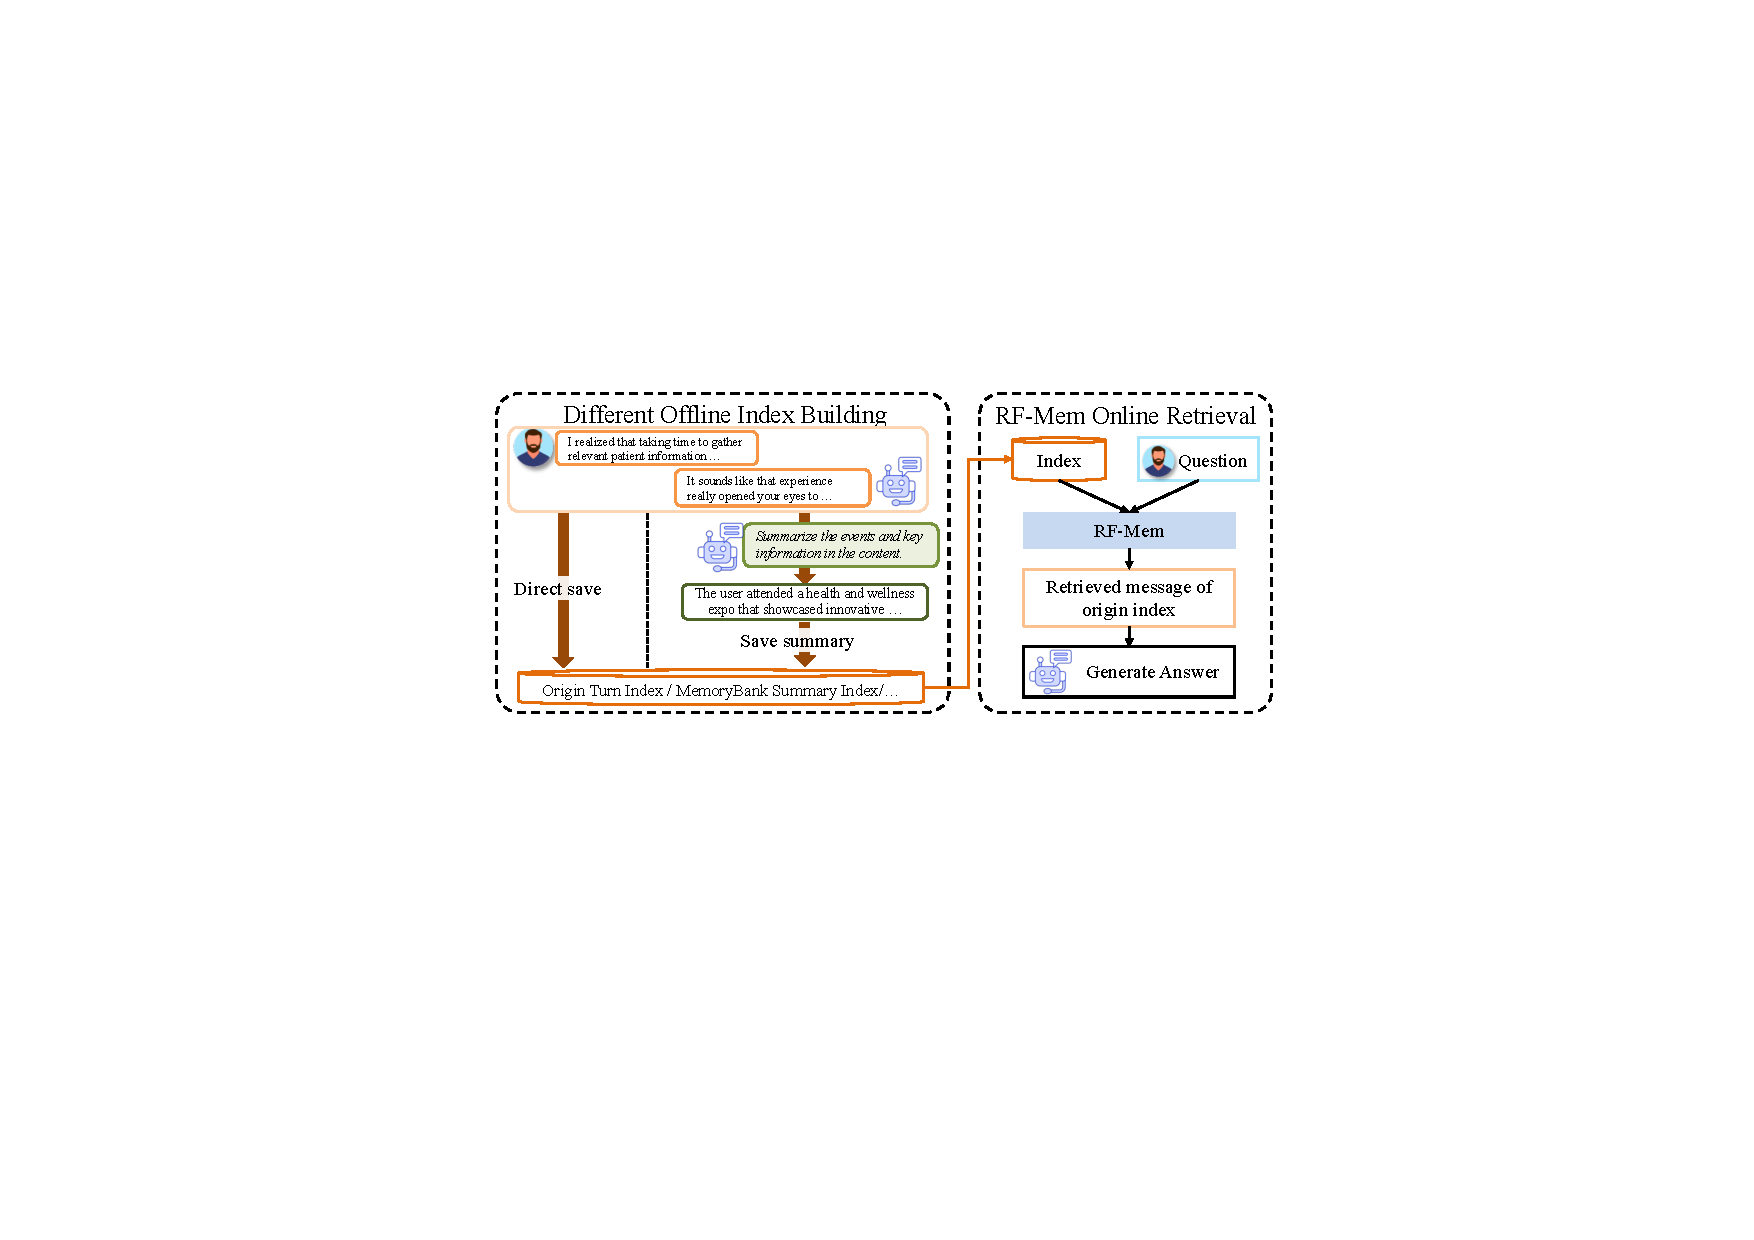
\includegraphics[width=0.90\linewidth]{chapter/figure/adaptive_study.pdf}
    \caption{Illustration of adaptive study setup. Offline indexes (e.g., MemoryBank or origin memory) provide different storage, while RF-Mem serves as an online retrieval layer that adapts to them.}
    % This design shows that RF-Mem complements, rather than replaces, existing indexing methods.
    \label{fig:adaptive_study}
\vspace{-10pt}
\end{figure}




\begin{table}[h]
\centering
\small
\caption{Results by using MemoryBank summary index on PersonaMem (32K corpus).}
\label{tab:adaptivity}
\setlength{\tabcolsep}{2pt}
\renewcommand{\arraystretch}{0.9}
\begin{tabular}{p{1.8cm}|M{1.2cm}|M{1.3cm}M{1.4cm}M{0.9cm}M{1.1cm}M{1.3cm}M{1.1cm}M{1.0cm}|>{\columncolor{blue!5}}c}
    \toprule
     \textbf{Method} & \textbf{Avg. Tokens}&\textbf{Revisit Reasons} & \textbf{Track Evolution} & \textbf{Latest Prefs} & \textbf{Aligned Recs} & \textbf{New Scenarios}& \textbf{Shared Facts} & \textbf{New Ideas} & \textbf{Overall}  \\
\midrule
% \rowcolor{gray!15}
% \multicolumn{10}{c}{\textbf{Origin turn-level index}} \\
% Familiarity   & 3515.9 & 0.9091 & 0.6475 & 0.6471 & 0.6364 & 0.5614 & 0.5426 & 0.2151 & 0.5908 \\
% Recollection  & 3711.1 & 0.9495 & 0.6547 & 0.7059 & 0.7818 & 0.5965 & 0.5194 & 0.2688 & 0.6214 \\
% RF-Mem        & 3566.6 & 0.9495 & 0.6619 & 0.7059 & 0.7818 & 0.6140 & 0.5659 & 0.2688 & \textbf{0.6350} \\
% \midrule
\rowcolor{gray!15}
\multicolumn{10}{c}{\textbf{MemoryBank summary index}} \\
Familiarity   & 1267.6 & 0.7475 & 0.6187 & 0.5882 & 0.5818 & 0.3333 & 0.4341 & 0.1505 & 0.4941 \\
Recollection  & 1441.8 & 0.8182 & 0.6259 & 0.5294 & 0.6909 & 0.4737 & 0.4031 & 0.1398 & 0.5212 \\
RF-Mem        & 1421.8 & 0.8384 & 0.6259 & 0.5294 & 0.6545 & 0.4211 & 0.4419 & 0.1828 & \textbf{0.5314} \\
\bottomrule
\end{tabular}
\vspace{-10pt}
\end{table}

To further examine the modularity of RF-Mem, we integrate it with external indexing schemes beyond raw turn-level memory. As shown in Figure~\ref{fig:adaptive_study}, offline methods such as \emph{MemoryBank}~\citep{zhong2024memorybank} first summarize user dialog into indexes (e.g., turn-level summaries), while RF-Mem operates as an online module during retrieval. This separation of offline indexing and online retrieval highlights that RF-Mem does not compete with summarization- or graph-based memory banks, but instead complements them by enabling human-like remembering. Table~\ref{tab:adaptivity} highlights that RF-Mem demonstrates robustness across both settings: it achieves the highest overall accuracy under the turn-level index, and crucially, it narrows the performance drop under the summary index compared to single-path baselines. 
This adaptivity confirms that RF-Mem is modular and can be layered on top of heterogeneous memory indices, providing an uncertainty-aware dual-process retrieval mechanism that complements, rather than replaces, external indexing methods.

\subsubsection{\revise{Adaptive to Query Expansion Method}}

\begin{figure}[h]
    \centering
    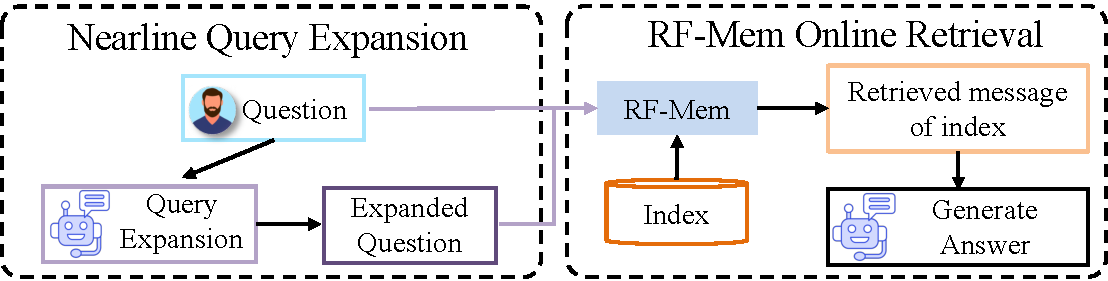
\includegraphics[width=0.9\linewidth]{chapter/figure/Query_expansion.pdf}
    \caption{\revise{Illustration of the adaptive study setup. Nearline query expansion (e.g., HyDE) enriches the query representation, and RF-Mem operates as the online retrieval layer.}}
    \label{fig:adaptive_query_study}
\vspace{-10pt}
\end{figure}

\begin{table}[ht]
\vspace{-10pt}
\centering
\small
\caption{\revise{Results by using HyDE query expansion method on PersonaBench.}}
\label{tab:adaptive_query_study}
\setlength{\tabcolsep}{1pt}
\renewcommand{\arraystretch}{0.8}
    \begin{tabular}{p{1.3cm}|M{1.2cm}M{1.2cm}M{1.2cm}M{1.2cm}>{\columncolor{blue!5}}M{1.1cm}
                            |M{1.2cm}M{1.2cm}M{1.2cm}M{1.2cm}>{\columncolor{blue!5}}M{1.1cm}}
        \toprule
        \textbf{Metrics}  &
        \multicolumn{5}{c|}{\textbf{Recall@5}} &
        \multicolumn{5}{c}{\textbf{Recall@10}} \\
        \cmidrule(lr){2-6} \cmidrule(l){7-11}
        \textbf{HyDE}
        & \textbf{Basic Info} & \textbf{Social Info} & \textbf{Pref Easy} & \textbf{Pref Hard} & \textbf{Overall}
        & \textbf{Basic Info} & \textbf{Social Info} & \textbf{Pref Easy} & \textbf{Pref Hard} & \textbf{Overall}   \\
        \midrule
        \rowcolor{gray!15}
        \multicolumn{11}{c}{\textit{multi-qa-MiniLM-L6-cos-v1}} \\
        Famili. & 0.3106 & 0.3909 & 0.4615 & 0.3122 & 0.3464 & 0.5000 & 0.4991 & 0.5737 & 0.5220 & 0.5120 \\
        Recol.  & 0.3015 & 0.4135 & 0.4615 & 0.3171 & 0.3482 & 0.4909 & 0.5028 & 0.5929 & 0.4878 & 0.5046 \\
        RF-Mem  & 0.3061 & 0.4135 & 0.4615 & 0.3171 & \textbf{0.3504} & 0.5091 & 0.5028 & 0.5929 & 0.5220 & \textbf{0.5194} \\
        \bottomrule
        \end{tabular}
\vspace{-10pt}
\end{table}

\revise{To further assess the adaptability of RF-Mem, we combine nearline query expansion with online retrieval and examine their interaction on PersonaBench. As illustrated in Figure~\ref{fig:adaptive_query_study}, the nearline expansion methods we adopt, HyDE~\citep{gao2023precise}, generate pseudo-relevance feedback that enriches the original query. RF-Mem then operates as an online retrieval layer.
Table~\ref{tab:adaptive_query_study} reports the results when applying HyDE-based expansion. Across all categories, RF-Mem consistently matches or surpasses Familiarity baselines, demonstrating that its dual-process mechanism remains effective even when the upstream query representation shifts.
These findings confirm that RF-Mem is modular and can be seamlessly integrated into nearline expansion pipelines. 
% Rather than replacing expansion-based methods, RF-Mem complements them by providing an uncertainty-aware retrieval controller.
}


\subsubsection{\revise{Adaptive to Iterative RAG Method}}

\begin{figure}[h]
    \centering
    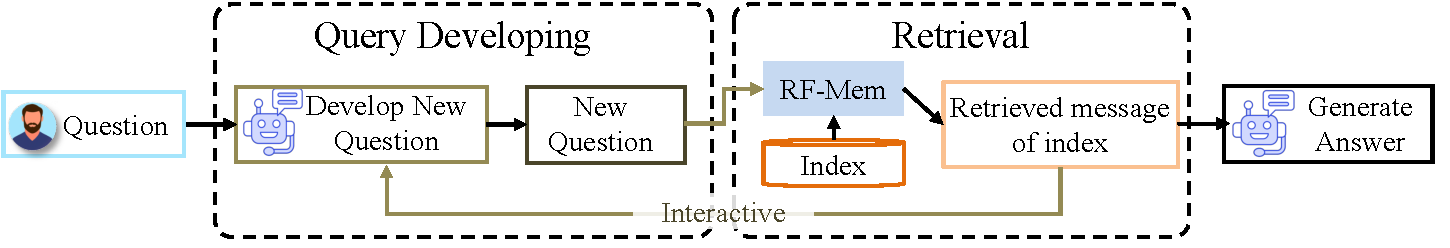
\includegraphics[width=0.90\linewidth]{chapter/figure/Iteractive.pdf}
    \caption{\revise{Illustration of adaptive study setup. Iterative RAG (e.g., Search-o1) provides a multi-turn retrieval for answer generation, while RF-Mem serves as the retrieval layer that adapts to it.}}
    \label{fig:adaptive_inter_study}
\vspace{-10pt}
\end{figure}

\revise{To further evaluate the adaptability of RF-Mem under iterative retrieval settings, we pair it with a multi-turn reasoning pipeline based on Search-o1~\citep{li2025search}. As illustrated in Figure~\ref{fig:adaptive_inter_study}, Search-o1 develops refined follow-up queries through iterative question generation, while RF-Mem functions as the retrieval layer that reacts to these evolving queries in real time. 
Table~\ref{tab:adaptive_inter_study} summarizes results using the Search-o1 interactive retrieval on the PersonaMem. RF-Mem still achieves the highest overall score. These findings demonstrate that RF-Mem retains its effectiveness in iterative RAG settings. 
% Instead of competing with multi-turn reasoning frameworks such as Search-o1, RF-Mem complements them by providing an adaptive, uncertainty-aware retrieval mechanism that stabilizes retrieval across evolving query states.
}

\begin{table}[h]
\centering
\small
\caption{\revise{Results by using Search-o1 iterative retrieval on PersonaMem (32K corpus).}}
\label{tab:adaptive_inter_study}
\setlength{\tabcolsep}{2pt}
\renewcommand{\arraystretch}{0.8}
\begin{tabular}{p{1.8cm}|M{1.2cm}|M{1.3cm}M{1.4cm}M{0.9cm}M{1.1cm}M{1.3cm}M{1.1cm}M{1.0cm}|>{\columncolor{blue!5}}c}
    \toprule
     \textbf{Search-o1} & \textbf{Avg. Tokens}&\textbf{Revisit Reasons} & \textbf{Track Evolution} & \textbf{Latest Prefs} & \textbf{Aligned Recs} & \textbf{New Scenarios}& \textbf{Shared Facts} & \textbf{New Ideas} & \textbf{Overall}  \\
\midrule
\rowcolor{gray!15}
\multicolumn{10}{c}{\textbf{Search-o1}} \\
Familiarity  & 4948.7 & 0.8687 & 0.6259 & 0.5882 & 0.6545 & 0.5614 & 0.5271 & 0.2581 & 0.5823 \\
Recollection & 5103.9 & 0.8990 & 0.6619 & 0.6471 & 0.7091 & 0.5789 & 0.4961 & 0.2796 & 0.6010 \\
RF-MEM       & 5158.2 & 0.9293 & 0.6978 & 0.6471 & 0.7455 & 0.5789 & 0.5349 & 0.2043 & \textbf{0.6146} \\
\bottomrule
\end{tabular}
\vspace{-10pt}
\end{table}




% \subsection{Parameter sensitivity}

% \begin{figure}[t]
%     \centering
%     \includegraphics[width=0.95\linewidth]{iclr2026/chapter/figure/heatmaps_alpha_tau.pdf}
%     \caption{Sensitivity of RF-Mem to hyperparameters $\alpha$ (query mixing) and $\tau$ (entropy threshold) on PersonaMem (Accuracy) and PersonaBench (Recall@5).}
%     \label{fig:alpha-tau}
% \end{figure}

% To further examine the robustness of RF-Mem, we conduct a sensitivity analysis on the two central hyperparameters: the query mixing coefficient $\alpha$ and the entropy threshold $\tau$. As shown in Figure~\ref{fig:alpha-tau}, both PersonaMem and PersonaBench results exhibit stable performance across a broad range of settings. 

% \textbf{Effect of query mixing coefficient $\alpha$.}
% We first examine the role of $\alpha$, which controls the balance between preserving the original query and incorporating cluster centroids during refinement. 
% As shown in Figure~\ref{fig:alpha-tau}, performance improves with moderate values ($0.7$–$0.8$), indicating that partial blending is critical: overly high $\alpha$ reduces exploration to surface-level similarity (Familiarity-like), while overly low $\alpha$ overemphasizes centroid feedback, diluting the query intent. 
% This confirms that controlled mixing enables effective contextual reconstruction, consistent with the theoretical view of recollection as a cue-guided extension of initial recognition.  

% \textbf{Effect of entropy threshold $\tau$.}
% We then evaluate $\tau$, which governs the switch between Familiarity and Recollection. 
% The results show that mid-range thresholds ($0.4$–$0.6$) deliver the most stable gains across both PersonaMem and PersonaBench. 
% A very low $\tau$ prematurely activates Recollection, leading to redundant expansion and efficiency loss, while a very high $\tau$ locks the system in Familiarity mode, missing opportunities for deeper reasoning. 
% This pattern aligns with dual-process theory: effective memory retrieval arises when the system adapts its depth of search according to uncertainty, rather than committing to either mode exclusively.  